\chapter{Introducción}
Si el universo tuvo un principio, como el \textit{Big Bang}, procedente de esa ``explosión'' la distribución de materia y energía habría sido muy irregular. Enormemente difusa. El tiempo y el espacio habrían estado curvados, retorcidos, deformados.

Pero cuando miramos al universo hoy, no vemos nada de eso. La distribución de materia y energía es casi uniforme en el universo, y el propio espacio es extremadamente plano, obedeciendo a las leyes de la geometría más sencilla. Así que, ¿cómo llegamos desde ese salvaje estado inicial hasta el presente? Ahí es donde nació la idea de inflación.

El concepto que introdujo la inflación es que, después del \textit{Big Bang}, quizás hubo un periodo de expansión muy rápida y acelerada, expandiendo el universo tan rápido que lo convertiría en algo aplanado y uniforme, y la distribución de materia y energía habría sido también uniformada de esta manera.

La teoría inflacionaria, uno de los ejes centrales de la Cosmología moderna, fue introducida por Alan Guth ---entre otros--- en 1981 para resolver una serie de problemas~\cite{peebles1993principles} que estaban presentes en el marco teórico de la Cosmología de la época: el \textit{Hot Big Bang}. En la~\autoref{fig::guth} se muestra una parte de sus notas originales.
\begin{figure}[t]
    \centering
    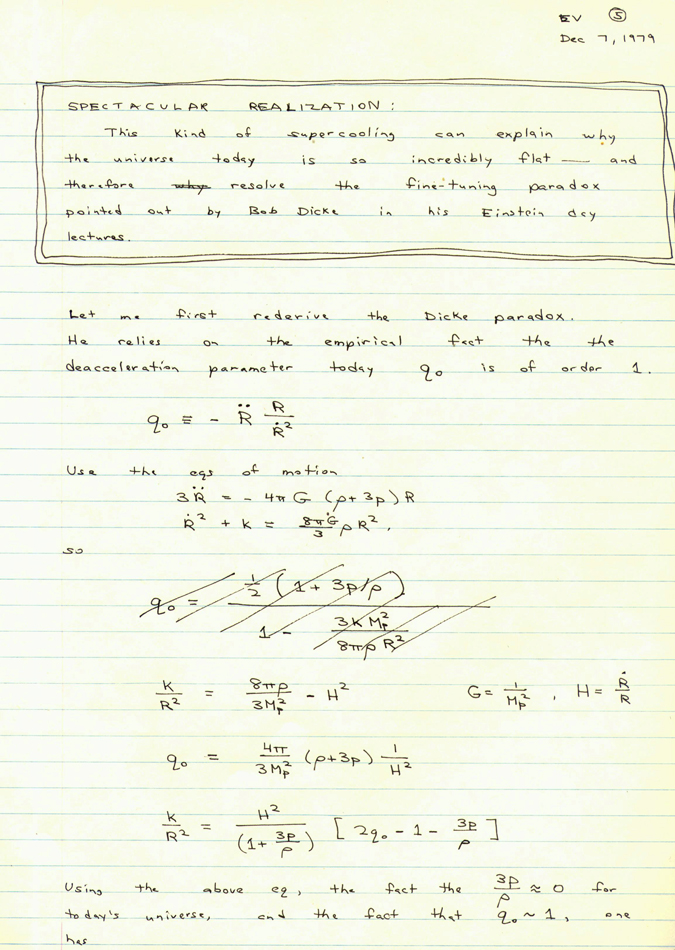
\includegraphics[scale=.85]{img/AlanGuth.jpg}
    \caption{Cuaderno con la idea original de Guth}
    \label{fig::guth}
\end{figure}

La teoría del \textit{Hot Big Bang} es considerablemente exitosa, superando algunas pruebas clave de observación: expansión del Universo, la existencia y espectro del CMB (\textit{Cosmic Microwave Background}), las abundancias de elementos ligeros en el Universo (nucleosíntesis), entre otras~\cite{liddle1998introduction}. Aun así, surgen dilemas en esta teoría ya que se limita a aquellas épocas en las que el Universo es lo suficientemente frío para que los procesos físicos fundamentales que subyacen estén bien consolidados y comprendidos a través de la experiencia en la Tierra; no aborda el estado del Universo en momentos anteriores, más calientes.
\newpage
Estas cuestiones cruciales sin respuesta en el \textit{Hot Big Bang} ---precursoras en la introducción de la inflación--- son el problema de la \textbf{planitud}, el problema del \textbf{horizonte} y la existencia de \textbf{monopolos magnéticos}. Tanto la primera como la segunda son el objeto de estudio de este texto y están relacionadas con las condiciones iniciales del Universo, que tuvieron que ser muy especiales y finamente ajustadas para dar lugar a lo que se observa hoy día.

Para especificar las condiciones iniciales del \textit{Hot Big Bang}, se definen las posiciones y velocidades de todas las partículas en un intervalo de tiempo inicial. Las leyes de la gravedad se utilizan entonces para hacer evolucionar el sistema en el tiempo. En la teoría estándar del \textit{Big Bang} se supone la distribución de materia como homogénea e isotrópica~\cite{baumann2022cosmology}. Pero, ¿cómo se explica esta uniformidad del Universo temprano? Incluso es algo que contrasta con la imagen proyectada por la teoría del \textit{Big Bang} donde la mayor parte del Universo parece no haber estado en contacto causal y no hay motivo dinámico para que estas regiones causalmente no conectadas tengan tales propiedades físicas similares que se suponen. Este problema de la homogeneidad se conoce como el problema del \textbf{horizonte}.

Para visualizar el primer problema, considérense dos direcciones opuestas en el cielo. Los fotones del CMB que recibimos de dichas direcciones fueron emitidos en los puntos etiquetados como \(q\) y \(p\) en la~\autoref{fig::horizonproblem}. Se observa que los fotones fueron liberados lo suficientemente cerca de la singularidad del Big Bang para que los conos de luz del pasado de \(q\) y \(p\) no se superpongan. Como ningún punto se encuentra dentro de los horizontes de \(q\) y \(p\), tenemos el siguiente enigma: ¿Cómo ``saben'' los fotones procedentes de estos dos puntos que deben estar a la misma temperatura? Simplemente no hubo tiempo suficiente para que las diferencias en las temperaturas iniciales se eliminaran mediante transferencia de calor. Lo mismo se aplica para cualesquiera dos puntos en el CMB que estén separados por más de 2°~\cite{baumann2022cosmology}.
\begin{figure}[t]
    \centering
    \def\svgwidth{0.75\textwidth}
    \input{svg/horizonproblem.pdf_tex}
    \caption[Ilustración del problema del horizonte]{Ilustración del problema del horizonte en el modelo convencional del Big Bang. Todos los eventos que observamos actualmente están en nuestro cono de luz pasado. La intersección de nuestro cono de luz del pasado con la franja espacial en el momento de la recombinación es la superficie de última dispersión. Los puntos que están separados por más de 2° en el cielo parecen no haber estado nunca haber estado en contacto causal, ya que sus conos de luz pasados no se solapan.}
    \label{fig::horizonproblem}
\end{figure}

Para que el universo siga siendo homogéneo en tiempos posteriores, las velocidades iniciales deben tomar valores muy precisos. Si las velocidades iniciales son ligeramente demasiado pequeñas, el Universo vuelve a colapsar en una fracción de segundo. Si son demasiado grandes, el Universo se expande demasiado rápido y se queda casi vacío. El ajuste de las velocidades iniciales se hace aún más drástico si se considera en combinación con el problema del horizonte, ya que las velocidades de las partículas deben ajustarse a través de regiones del espacio causalmente desconectadas. Este ajuste preciso en la condición inicial de velocidad es lo que se conoce como el problema de la \textbf{planitud} y se plantea comúnmente como por qué la curvatura espacial del Universo es tan pequeña, cuya relación con las velocidades viene dada por la suma de la energía cinética y potencial en una determinada región~\cite{baumann2022cosmology}.

Inflación predice que las condiciones iniciales del universo son descritas con buena aproximación por un campo aleatorio gaussiano~\cite{baumann2022cosmology,dodelson2020modern}.